\documentclass[10pt]{article}

\usepackage{amsmath, amssymb}
\usepackage[margin=1in]{geometry}
\usepackage{enumitem}
\usepackage{tikz}
\usetikzlibrary{shapes.geometric, backgrounds, calc}
\usepackage{calc}
\usepackage{multicol}

\usepackage{xcolor}
\definecolor{color1}{RGB}{0, 99, 178} % Electric Blue Lemonade
\definecolor{color2}{RGB}{193, 228, 242} % Sky Blue

\setlength{\parskip}{1ex}
\setlength{\parindent}{0pt}

\newlength{\topedge}
\newlength{\bottomedge}

% Section styling
\usepackage{titlesec, titletoc}
\titleformat{\section}[display]{}{}{0pt}{
    \bf \Large \color{white}
    \setlength{\topedge}{0.9\baselineskip}
    \setlength{\bottomedge}{-0.4\baselineskip}
    \begin{tikzpicture}[overlay, x=1in, y=1in]
        \fill[color1] (-1, \bottomedge) -- (6.5, \bottomedge) -- (6.2, \topedge) -- (-1, \topedge) -- cycle;
    \end{tikzpicture}%
}[]
\titlespacing*{\section}{0pt}{-3ex}{1ex} % remove some space before, add some after

% Subsection styling
\titleformat{\subsection}[display]{}{}{0pt}{
    \bf \large \color{white}
    \setlength{\topedge}{0.9\baselineskip}
    \setlength{\bottomedge}{-0.4\baselineskip}
    \begin{tikzpicture}[overlay, x=1in, y=1in]
        \fill[color1] (-1, \bottomedge) -- (2.75, \bottomedge) -- (2.5, \topedge) -- (-1, \topedge) -- cycle;
    \end{tikzpicture}%
}[]
\titlespacing*{\subsection}{0pt}{-2ex}{0pt} % remove some space before

\usepackage[colorlinks, linkcolor=color1, urlcolor=color1]{hyperref}

% change to \usepackage[sols]{../Documents/handout} to see solutions
% change to \usepackage[plan]{../Documents/handout} to see lesson plan and notes
\usepackage[]{../Documents/handout}

\usepackage{fdsymbol}
\setlist{itemsep=1ex, parsep=1ex, topsep=1ex}
\setlist[itemize]{label={\color{color1} $\smallblackdiamond$}}
\usepackage{tikz}
\usetikzlibrary{arrows}
\usepackage{pgfplots}

\pgfplotsset{compat = 1.16}

\begin{document}

\begin{center}
    
\begin{tikzpicture}
        \node (title) [trapezium, trapezium left angle=60, trapezium right angle=120, align=center, inner sep=10pt, fill=color1, text=white] at (0, 0) {\bf \LARGE Modeling with Functions};
        \node[trapezium, trapezium left angle=120, trapezium right angle=60, align=center, inner sep=6pt, fill=color2, text=black]
        at ($(title.top left corner) + (0,0.2)$) {\large Class 1};
        \node[trapezium, trapezium left angle=120, trapezium right angle=60, align=center, inner sep=6pt, fill=color2, text=black]
        at ($(title.bottom right corner) + (0,-0.2)$) {\large Mon, Sep.\ 8};
    \end{tikzpicture}
\end{center}

\begin{plan}
    \section{Lesson Plan}
    \vspace*{-4ex}
    
    \subsection{Administrative Notes}
    \begin{itemize}
        \item Course policies were already discussed during our big course meeting last Wednesday, so there's no need to go over the syllabus again. However, you should re-emphasize the importance of the collaborative, active classroom to students' learning, as well as the technology policy and the new grading scheme. Remind students about PSets and quiz sessions.
        \item Sectioning is still in flux, which means you may want to get a more accurate picture of who is in your section by printing out a roster and asking students to check off their names. Ultimately we will be taking attendance via a spreadsheet (you can have your CAs help with this) but we will be flexible the first week or so. 
       % \item Get students to join the Math 1a Slack to stay informed with announcements and ask questions.
        \item Make sure students are aware of office hours and MQC and why both of them are helpful. The first MQC session is from 7:30--9:30 PM on Monday evening (9/8), and office hours will start on Monday as well. 
        \item The first quiz sessions start on Tuesday, September 16. There will be a variety of times for quizzes from Tuesdays-Thursdays. Encourage students to attend, as they are a valuable source of review and self-testing. (They also get a PSet drop for every 4 they attend). They are free to attend any quiz session time (the schedule is on Canvas).
        \item The first PSet is due on Wednesday, September 10. Students should submit via Gradescope - the due time is 30 minutes before their section.
    \end{itemize}
    
    \subsection{Main Ideas}
    The primary goal of the first class is to begin establishing your classroom culture. This means students should be actively participating in group work from the very beginning. This is a useful time to establish some classroom norms around working together and respectfully sharing ideas, especially when there's confusion or mistakes. Whatever happens in the first few days of class will set the tone for the whole semester!
    
    The secondary goal of the first class is for students to practice using functions to model real-world scenarios.
    \begin{itemize}
        \item In the first two classes, it will become clear that students have varying levels of comfort working with functions. Emphasize that the goal of working in groups is not to finish the problem as fast as possible, but for every student to have a solid understanding.
        \item The general flow of these modeling problems is making a sketch $\rightarrow$ choosing an appropriate kind of function $\rightarrow$ refining the function using specific information from the problem. Some students will want to skip straight to the end and might get stuck trying to come up with a formula without anything to go on.
        \item Be sure to discuss the terms \emph{increasing}, \emph{decreasing}, \emph{concave up}, and \emph{concave down} at some point - you can do this when discussing the first problem.
        \item Students should already have at least a vague mental ``library'' of common types of functions and what their graphs look like. They will be recalling/adding to the library during the first two classes and PSets.
    \end{itemize}
    
    \subsection{My Plan} % Me = Hannah, Fall 2025
    \begin{itemize}
        \item I'll start by introducing myself to the class and having the CAs do the same.
        \item I'll spend some time going over basics of the course and  explaining the importance of group work to our class, then randomly assign groups of 3--4 students (I do this via numbered worksheets).
        \item In groups, students will do an icebreaker activity followed by some discussion of classroom norms. It's worth spending a fair amount of time on this! (I can go up to 30 min).
        \item I'll have all the groups find a place at the chalkboard to start working on \#1. There's a lot to talk about in this very simple situation---see the notes on the problem below.
        \item Then I'll have everyone work on \#2. As a class, we'll briefly discuss what everyone came up with for \#1 and why a linear model is appropriate.
        \item I don't expect to get to \#3, but it's there if groups really blast through \#2. I'll tell my students that most of the worksheets are intentionally longer that what we'll have time for in class. They can use any problems we don't get to for extra practice, comparing their work with the worksheet solutions posted on Canvas. We may need to reiterate this in the first week or so!
    \end{itemize}
    
    \section{Worksheet}
    \vspace*{0.8cm}
\end{plan}

\vspace*{-0.8cm}
\begin{center}
    \hspace*{-1in}
    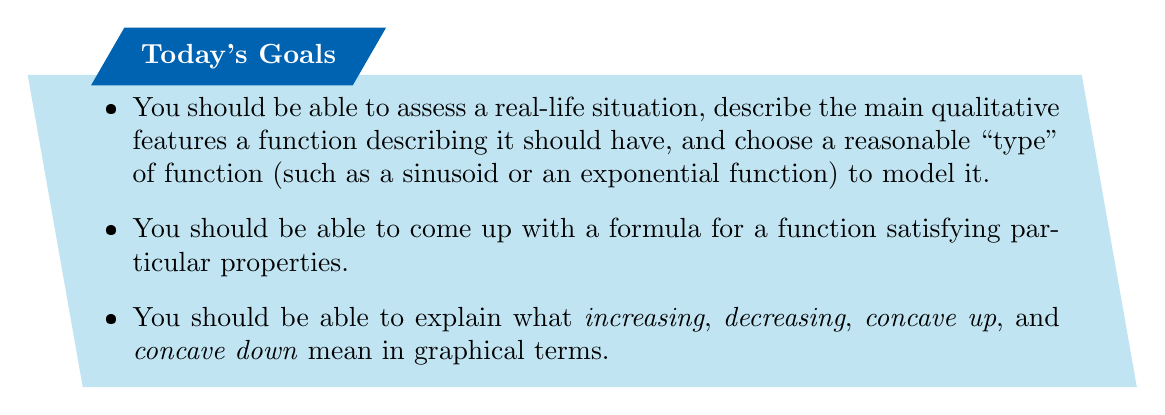
\begin{tikzpicture}
        \node (goals) [trapezium, trapezium left angle=100, trapezium right angle=80, align=center, inner sep=8pt, fill=color2, text=black] at (0, 0)
            {\begin{minipage}{\textwidth} \begin{itemize}[leftmargin=*]
                \item You should be able to assess a real-life situation, describe the main qualitative features a function describing it should have, and choose a reasonable ``type'' of function (such as a sinusoid or an exponential function) to model it.
                \item You should be able to come up with a formula for a function satisfying particular properties.
                \item You should be able to explain what \emph{increasing}, \emph{decreasing}, \emph{concave up}, and \emph{concave down} mean in graphical terms.
            \end{itemize} \end{minipage}};
            
        \node[trapezium, trapezium left angle=60, trapezium right angle=120, align=center, anchor=bottom left corner, inner sep=6pt, fill=color1, text=white] at ($(goals.top left corner) + (0.8, -0.15)$) {\bf Today's Goals};
    \end{tikzpicture}
    \hspace*{-1in}
\end{center}

\begin{enumerate}[leftmargin=*]

\item
    \begin{note}
        There are lot of points worth discussing here:
        
        \begin{itemize}
            \item Whether the function ought to be increasing or decreasing.
            \item Whether the function ought to be concave up or concave down (and
            what it is about the situation that tells you that).  Since we
            haven't talked about slope as rate of change yet, I'll probably talk
            instead about successive small changes: in one minute, you expect
            the temperature to decrease by some amount; in the next minute, you
            expect a slightly smaller decrease, which is what makes the graph
            curve.  We could summarize this as ``decreasing at a slowing rate''.
            (I avoid the phrasing ``decreasing at an increasing/decreasing
            rate'' since students tend to find it ambiguous.)
            \item The long-term behavior of the function.
            \item There are different functions that match the qualitative
            features above: $A + B e^{-kt}$, $A + \frac{B}{t + 1}$, etc. You
            can let students know that a model like this can be refined by
            taking data or appealing to principles of physics.
            \item For part (b), they should
            have some idea of reasonable values for the long-term behavior and
            starting temperature; how would these affect their function?  (There
            are many possible ways you could approach this discussion; they
            might think of starting with a basic function like $e^{-t}$ and
            stretching and shifting it, or they might think of starting with a
            general family like $A + B e^{-t}$ and solving for the parameters in
            it.) 
        \end{itemize}
    \end{note}

    One morning, Aida brews a hot cup of coffee but then forgets to drink it. 
    \begin{enumerate}
        \item 
        \begin{problem}[\vfill] 
            Sketch a graph of the coffee's temperature over time (starting right after she's finished brewing it).
            Describe the shape of the graph using mathematical language and explain why that shape is appropriate.
        \end{problem} 
        \begin{solution} 
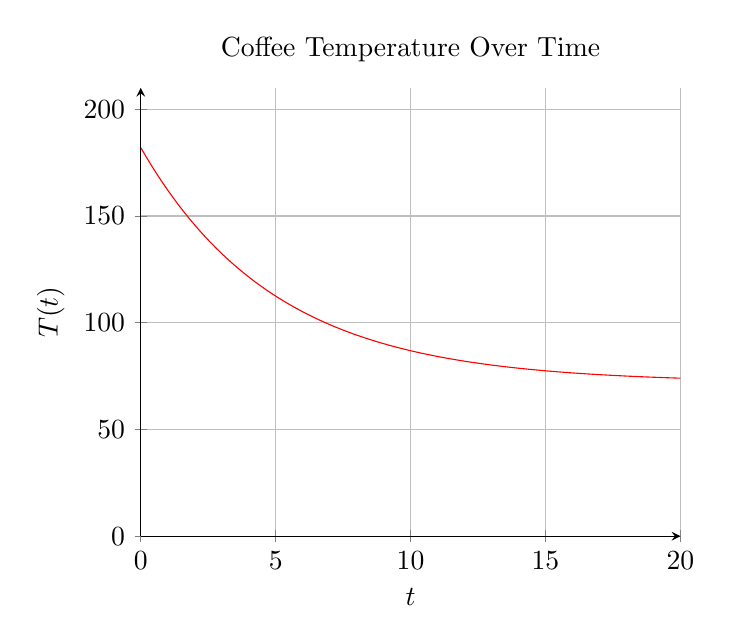
\begin{tikzpicture}
\begin{axis}[
    axis lines = left,
    xlabel = \(t\),
    ylabel = \(T(t)\),
    ymin = 0, ymax = 210,
    xmin = 0, xmax = 20,
    grid = major,
    title = {Coffee Temperature Over Time},
]
\addplot [
    domain=0:20, 
    samples=100, 
    color=red,
    ] {72 + 110 * exp(-0.2*x)};
 \end{axis}
\end{tikzpicture}


In one minute, you expect the temperature to decrease by some amount; in the next minute, you
            expect a slightly smaller decrease, which is what makes the graph
            curve.  We could summarize this as ``decreasing at a slowing rate''.
            
\vspace{1ex}
\section{Increasing and Decreasing Functions}

\subsection{Increasing Functions}

An increasing function is one where the output (or ``y-value'') rises as the input (or ``x-value'') rises. In other words, as you move from left to right along the function, the graph goes up

Mathematically, a function \( f(x) \) is said to be increasing on an interval \( [a, b] \) if for any \( x_1 \) and \( x_2 \) within that interval,
\[
x_1 < x_2 \Rightarrow f(x_1) < f(x_2)
\]

\subsection{Decreasing Functions}

A decreasing function is the opposite of an increasing function. As you move from left to right along the function, the graph goes down.

Mathematically, a function \( f(x) \) is said to be decreasing on an interval \( [a, b] \) if for any \( x_1 \) and \( x_2 \) within that interval,
\[
x_1 < x_2 \Rightarrow f(x_1) > f(x_2)
\]

\section{Concave Up and Concave Down Functions}

\subsection{Concave Up}
Functions that have an increasing rate of change are called concave up. 

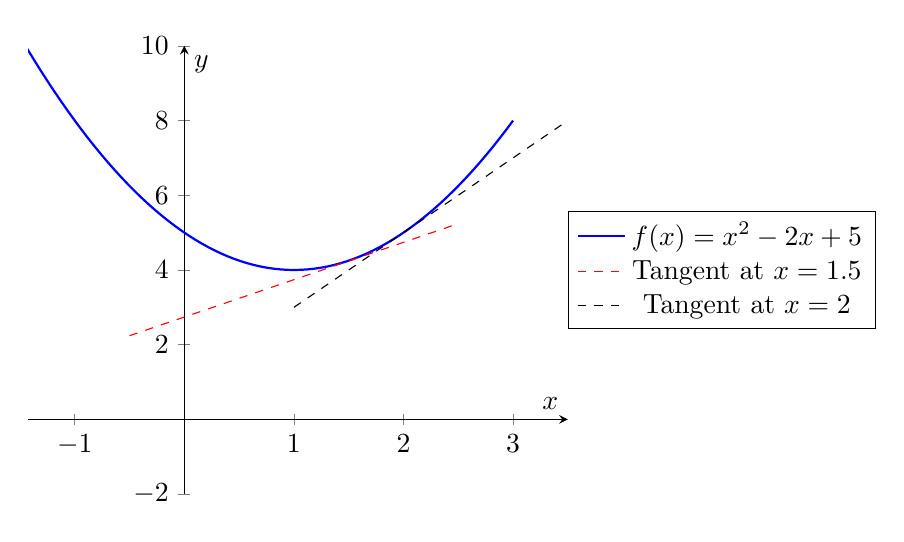
\begin{tikzpicture}
    \begin{axis}[
        axis lines = middle,
        xlabel = \(x\),
        ylabel = {\(y\)},
        domain = -3:3,
        samples = 100,
        ymin = -2,
        ymax = 10,
        legend style ={at={(1,0.5)},anchor=west}
    ]
    
    % Add a curve (e.g., y = x^2)
    \addplot[blue, thick]{ x^2-2*x +5};
    \addlegendentry{\(f(x) = x^2-2x +5\)}
    
    % Add the first tangent line at x = -1
    \addplot[dashed, red, domain=-.5:2.5]{(x -1.5 1) + 1.5^2-3+5};
    \addlegendentry{Tangent at \(x = 1.5\)}
    
    % Add the second tangent line at x = 1
    \addplot[dashed, black, domain=1:3.5]{2*1*(x - 2) + 2^2-4+5};
    \addlegendentry{Tangent at \(x = 2\)}
    
    \end{axis}
\end{tikzpicture}
\subsection{Concave Down}
Conversely, functions that have a decreasing rate of change are called concave down. 

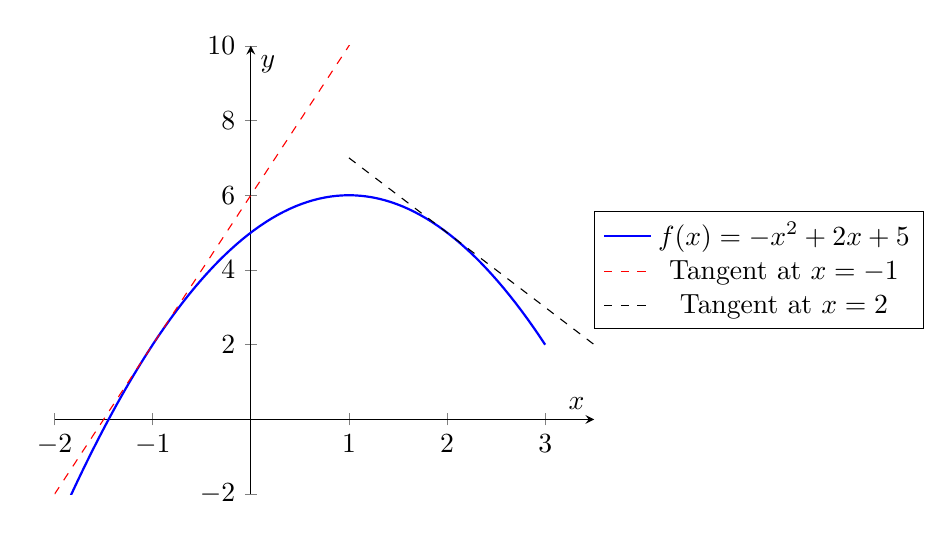
\begin{tikzpicture}
    \begin{axis}[
        axis lines = middle,
        xlabel = \(x\),
        ylabel = {\(y\)},
        domain = -3:3,
        samples = 100,
        ymin = -2,
        ymax = 10,
        legend style ={at={(1,0.5)},anchor=west}
    ]
    
    % Add a curve (e.g., y = -x^2)
    \addplot[blue, thick]{ -x^2 + 2*x +5};
    \addlegendentry{\(f(x) = -x^2+2x +5\)}
    
    % Add the first tangent line at x = -1
    \addplot[dashed, red, domain=-2:2.5]{2+4*(x+1)};
    \addlegendentry{Tangent at \(x = -1\)}
    
    % Add the second tangent line at x = 2
    \addplot[dashed, black, domain=1:3.5]{-2*(x - 2) + -2^2+4+5};
    \addlegendentry{Tangent at \(x = 2\)}
    
    \end{axis}
\end{tikzpicture}

So we see that our cooling function is decreasing and concave up.
\end{solution}
        \item
        \begin{problem}[\vfill \newpage]
            Try writing a formula for a function that looks like your sketch.
            This function would be a plausible model for this situation.
        \end{problem}
    \end{enumerate}




\begin{solution}
There are various functions that could match the qualitative features of a cooling cup of coffee, such as \( A + B e^{-kt} \) and \( A + \frac{B}{t + 1} \). However, the exponential decay function \( A + B e^{-kt} \) is commonly used for modeling cooling processes. You could see why this is a good choice by taking more data or  appealing to principles of physics.
\begin{itemize}
\item To build intuition, you can manipulate these parameters using \href{https://www.desmos.com/calculator/tdh4ybzztn}{Desmos}. Understanding the parent function \( F(t) = e^t \) is also crucial. The function \( A + B e^{-kt} \) can be viewed as a series of graph transformations: \( e^{-kt} \) reflects \( e^t \) over the \( y \)-axis and then horizontally compresses it by a factor of \( k \). The \( B \) term vertically stretches the function, and \( A \) vertically translates it.

\item The parameter \( A \) should represent the ambient room temperature. For example, let's assume \( A = 72^\circ \text{F} \).

\item We can assume that right after Aida brews the coffee, its temperature is around $190^\circ \text{F}$. Therefore, \( f(0) = 190^\circ \text{F} = A + B \). Solving for \( B \), we find \( B = 118^\circ \text{F} \).

\item Finally, the parameter \( k \) describes how quickly the coffee cools and depends on various factors like the material of the mug. Assuming that after 15 minutes the coffee cools to $100^\circ \text{F}$, we can solve for \( k \) as follows:

\begin{align*}
f(15) &= 100^\circ \text{F} = 72^\circ \text{F} + 118^\circ \text{F} \cdot e^{-15k} \\
28^\circ \text{F} &= 118^\circ \text{F} \cdot e^{-15k} \\
\frac{28}{118} &= e^{-15k} \\
\ln \left( \frac{28}{118} \right) &= -15k \\
k &= -\frac{1}{15} \ln \left( \frac{28}{118} \right) \approx 0.01 
\end{align*}
\end{itemize}

So a reasonable model for our situation is that $$f(t) = 72 + 118\cdot e^{-.01 t}$$
\end{solution}


\item
    \begin{note}
        Hopefully students won't have too much trouble coming up with the function itself, so you can focus on asking about why a linear model makes sense here and what the slope and intercept mean in context. 
    \end{note}

    Jay lives in New York City, and he often takes taxis. Taxis charge a base fare, and then an additional charge for each additional mile. It costs him \$26 to take a cab from his apartment to work, which is 4 miles, and it costs \$11 to travel from work to the gym, which is a mile and a half. 
    \begin{enumerate}
        \item \label{5mile} 
        \begin{problem}[\vfill]
            How much do you think it would cost Jay to get from the gym back home, which is 5 miles?
            Give the best answer you can and identify and assumptions which you are making.
        \end{problem}
        \begin{solution} 
  
    To estimate the cost for Jay to travel 5 miles from the gym back to his home, we need to think about how the taxi company is charging for rides. Since taxis charge a base fare for getting into the cab and then an additional charge for each additional mile, the fare for traveling \(x\) miles in the cab is given by
    \[
    F(x) = ax + b
    \]
    
    We need to find the values of \(a\) and \(b\). We have two data points: \((4, 26)\) for the trip from home to work and \((1.5, 11)\) for the trip from work to the gym.
  
  We can find $a$ by calculating the slope of the line connecting those two points: 
  
  $$ m = \frac{y_2 -y_1}{x_2-x_1} = \frac{ 26 - 11}{4 - 1.5} = \frac{15}{2.5} = 6 \frac{\text{dollars}}{\text{mile} } $$
   
  This means for each additional mile Jay goes in the taxi, he will pay an additional \$ 6. 
    
    Substituting back into either equation to find \(b\), we get:
    \[
    b = 26 - 4 \cdot 6 = 26 - 24 = 2
    \]
    
    Therefore, the fare function \( F(x) \) is:
    \[
    F(x) = 6x + 2
    \]
    
    To find out how much it would cost Jay to get from the gym back home, which is 5 miles, we use this function:
    \[
    F(5) = 6 \cdot 5 + 2 = 30 + 2 = 32
    \]
    
    So, it would cost Jay \$32 to travel 5 miles from the gym back to his home.
   
   
 
\end{solution} 

        \item
        \begin{problem}[\vfill \newpage]
            Let $x$ represent that distance that Jay travels and let $y$ represent the cost of the ride.
            Write $y$ as a function of $x$ and sketch a graph of the function.
            Then explain clearly what the slope represents in the context of this situation.
        \end{problem}
        \begin{solution} 
   Note that the tactic in part (\ref{5mile}) is to find the general solution and then plug in 5. This means that we have already answered this question:
   
   $$y = 6x+2,$$
   \begin{center}
   \begin{tikzpicture}[scale=0.5] 
  % Axes
  \draw[->,thick] (-1,0) -- (10.5,0) node[right] {$x$};
  \draw[->,thick] (0,-1) -- (0, 10.5) node[above] {$y$};

  % Tick marks and labels on x-axis
  \foreach \x in {1,2,3,4,5,6,..., 10}
    \draw (\x,0) -- (\x,-0.2) node[below] {\x};

  % Tick marks and labels on y-axis
  \foreach \y in {1,2,...,10}
    \draw (0,\y) -- (-0.2,\y) node[left] {\y};

  % Line y = 6x + 2
  \draw[red, very thick, domain=-1:1.5] plot (\x,{6*\x+2});

\end{tikzpicture}
 \end{center}

   Sometimes it is much easier to work with a specific solution and try and generalize. 
        \end{solution} 
    \end{enumerate}

\item
    \begin{note}
        This problem does a nice job getting the students to describe different features of a graph. You can really push them here to make sure they are giving a complete graph with labeled axes and defined variables. This is what the prompt about approximating the height of the flagpole is getting at.
    \end{note}

    \begin{problem}[\vfill]
        With your group, draw a  graph that represents a flag being raised on a flagpole that gives the height of the flag in feet versus time in seconds. Label and scale your axes. Explain how you decided on the shape of the graph and use it to give an estimate of the height of the flagpole.
    \end{problem}
    \begin{solution} 
There are many ways to approach this problem. Below is one possible solution with a commentary that highlights important thinking and assumptions made. 

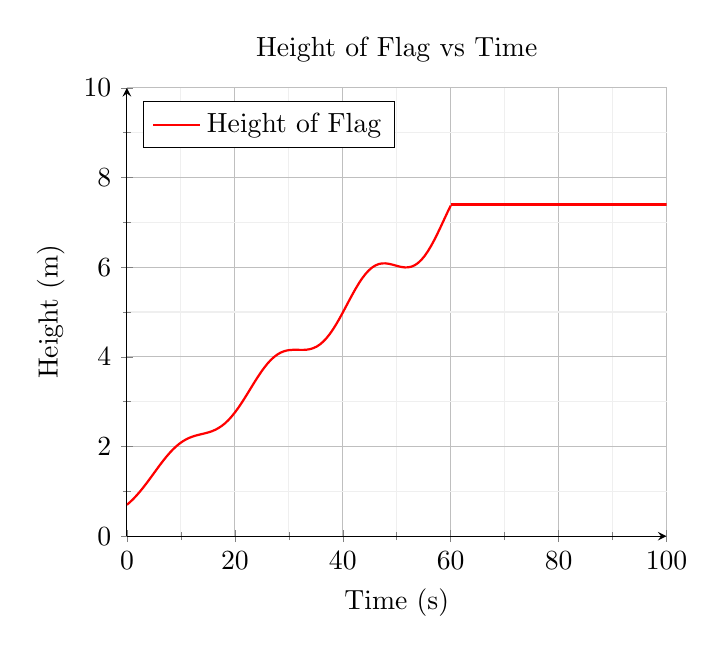
\begin{tikzpicture}
\begin{axis}[
    axis lines = left,
    xlabel = Time (s),
    ylabel = Height (m),
    title = {Height of Flag vs Time},
    xmin=0, xmax=100,
    ymin=0, ymax=10,
    grid=both,
    minor tick num=1,
    major grid style={lightgray},
    minor grid style={lightgray!25},
    legend pos=north west
]
\addplot[
    domain=0:60,
    samples=100,
    color=red,
    thick,
]
{.01*x*sin(x*10)*sin(x*10)+.1*x+sin(x*10)*sin(x*10)+.7*cos(x*10)*cos(x*10)}; 


\addplot[
    domain=60:100,
    samples=100,
    color=red,
    thick,
]
{7.4}; 

% Replace this with the function that you want to plot
\addlegendentry{Height of Flag}
\end{axis}

\end{tikzpicture}

\begin{itemize}
\item In this solution, the flag doesn't start at the ground. (Some cultures view it as a sign of disrespect for the flag to touch the ground.) So the y-intercept is not 0. 

\item The rate of at which the flag moves up the flag pole is not constant. It comes in bursts of progress followed by time for the person to grab the rope higher. Since the rate is not constant, the graph is not linear. We see that the concavity changes. 

\item Eventually, the flag gets to the top of the flag pole. This is reflected in the graph with the the horizontal line.
\end{itemize} 
\end{solution} 
\end{enumerate}

\end{document}